\documentclass[14pt, oneside]{altsu-report}
\title{Лабораторная работа №6 <<Разработка графической программы, моделирующую солнечную систему>>}
\author{Д.\,С.~Вебер, А.\,А.~Колесников}
\groupnumber{506}
\GradebookNumber{1337}
\supervisor{И.\,А.~Шмаков}
\supervisordegree{к.ф.-м.н., доцент}
\ministry{Министерство науки и высшего образования}
\country{Российской Федерации}
\fulluniversityname{ФГБОУ ВО Алтайский государственный университет}
\institute{Институт цифровых технологий, электроники и физики}
\department{Кафедра вычислительной техники и электроники}
\departmentchief{В.\,В.~Пашнев}
\departmentchiefdegree{к.ф.-м.н., доцент}
\shortdepartment{ВТиЭ}
\abstractRU{Объектом исследования данной работы является программный продукт, моделирующий солнечную систему. Программа написана на языке высокого уровня Python3 в среде разработки PyCharm Professional.

Разработанный продукт работает на компьютерах стандартной комплектации под операционными системами Linux.

Программный продукт предназначен для моделирования солнечной системы.}
%\abstractEN{Большой текст на английском!}
\keysRU{компьютерное моделирование, солнечная система}
%\keysEN{computer simulation, distributed version control}

\date{\the\year}

% Подключение файлов с библиотекой.
\addbibresource{graduate-students.bib}

\begin{document}
\maketitle

\setcounter{page}{2}
\makeabstract
\tableofcontents

\chapter*{Введение}
\addcontentsline{toc}{section}{Введение}
Цель работы заключается в том, чтобы разработать программу, которая будет моделировать солнечную систему, в которой мы проживаем. 

Задача состоит в том, чтобы работа выполнена командой с чёткий распределением ролей. Д.С.Вебер --- лидер проекта, А.А.Колесников --- кодировщик, тестировщик. 

В качестве парадигмы программирования было принято решение разрабатывать программу методом объектно-ориентированного программирования. Объектно-ориентированная парадигма была удобна для реализации операций над объектами, то есть нашими планетами, а также легче разобраться, что происходит в программе.   
\chapter{Глава 1. Инструменты}
\section{Раздел 1. Библиотеки}
В качестве основной графической библиотеки мы использовали Pygame~\cite{Pygame}. Это <<игровая библиотека>>, набор инструментов, помогающих программистам создавать игры. Выбор пал, ввиду приятного синтаксиса и подходящих инструментов разработки. Но при разработке мы столкнулись с такой проблемой, как отсутствие возможности создать второе окно с информацией о планете. Поэтому импортировали ещё одну графическую библиотеку под названием Tkinter. Tkinter --- кросс-платформенная событийно-ориентированная графическая библиотека на основе средств Tk, входящая в стандартную библиотеку языка программирования Python~\cite{Tkinter}. Для расчёта скоростей и траектории движения планет понадобился модуль math с арифметическими и тригонометрическими функциями. Чтобы происходило взаимодействие с операционной системой был импортирован модуль os.
\section{Раздел 2. Среда разработки}
В ходе работы были использованы разные текстовые редакторы кода, но в конце выбор пал на полноценную интегрированную среду разработку от JetBrains --- PyCharm Professional. PyCharm --- интегрированная среда разработки для языка программирования Python~\cite{Pycharm}. Предоставляет средства для анализа кода, графический отладчик, инструмент для запуска юнит-тестов.

\chapter{Глава 2. Ход работы}
\section{Раздел 1. Разработка}
Как было написано ранее разрабатывался программный продукт методом объектно-ориентированного программирования. Объектно-ориентированное программирование – это подход, при котором вся программа рассматривается как набор взаимодействующих друг с другом объектов. При этом нам важно знать их характеристики. У каждого объекта в системе есть свойства и поведение, как и у любого реального объекта. Такой подход помогает строить сложные системы более просто и естественно благодаря тому, что вся предметная область разбивается на объекты и каждый из них слабо связан с другими объектами. ООП позволяет упростить сложные объекты, составляя их из более маленьких и простых, поэтому над программой могут работать сотни разработчиков, каждый из которых занят своим блоком.

\begin{figure}[H]
\begin{center}
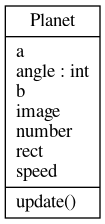
\includegraphics{uml} 
\caption{Диаграмма}
\end{center}
\end{figure}
\section{Раздел 2. Работа программы}
В ходе тестирования программы сбоев не было обнаружено. Программный продукт без проблем работает на любых компьютерах.
\begin{figure}[H]
\begin{center}
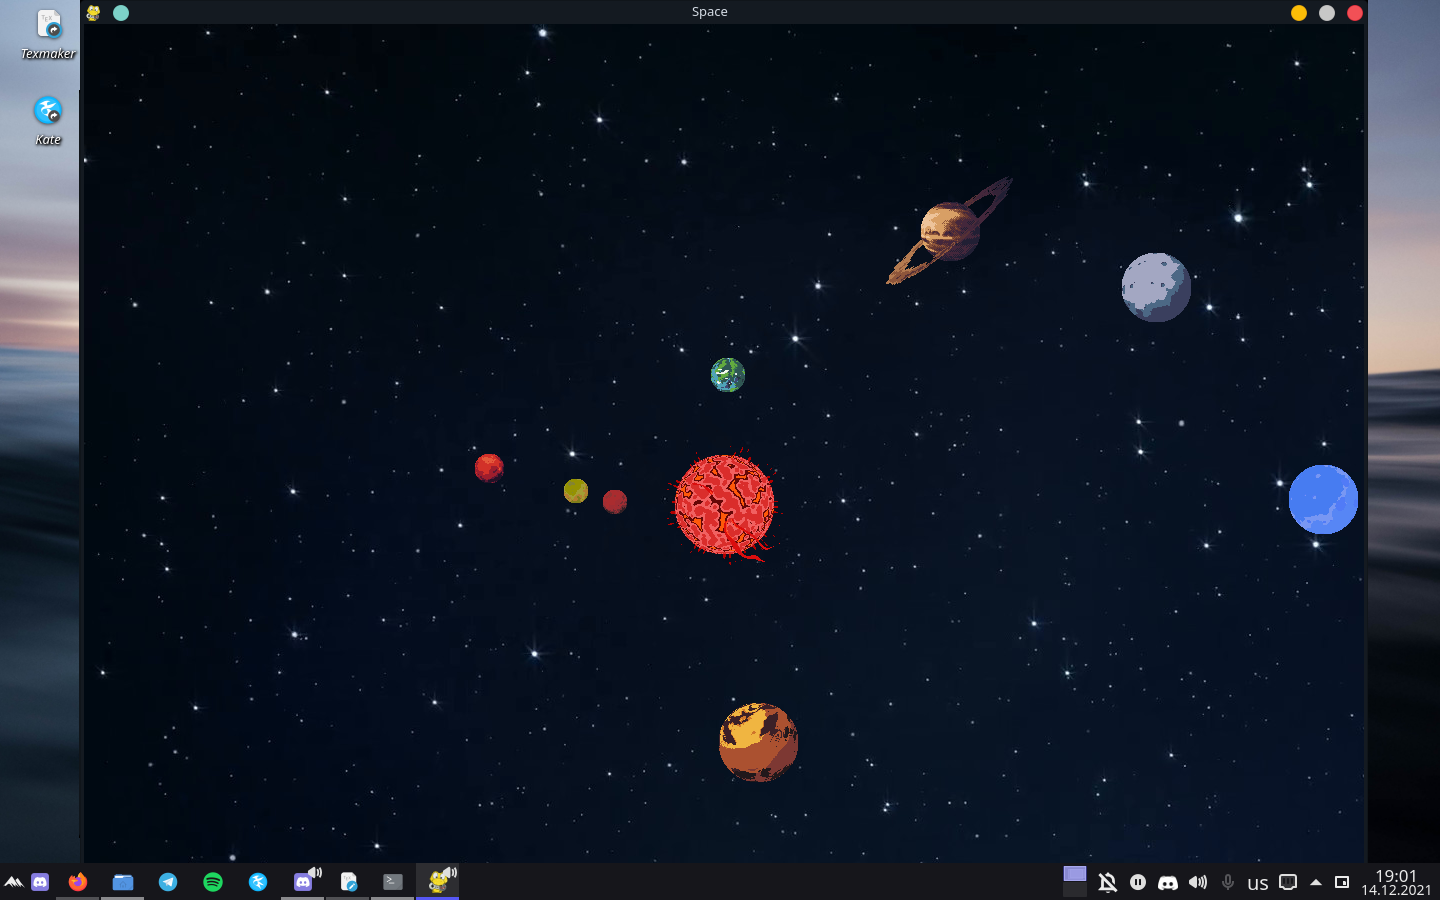
\includegraphics[scale=0.45]{test1} 
\caption{Тест}
\end{center}
\end{figure}
\begin{figure}[H]
\begin{center}
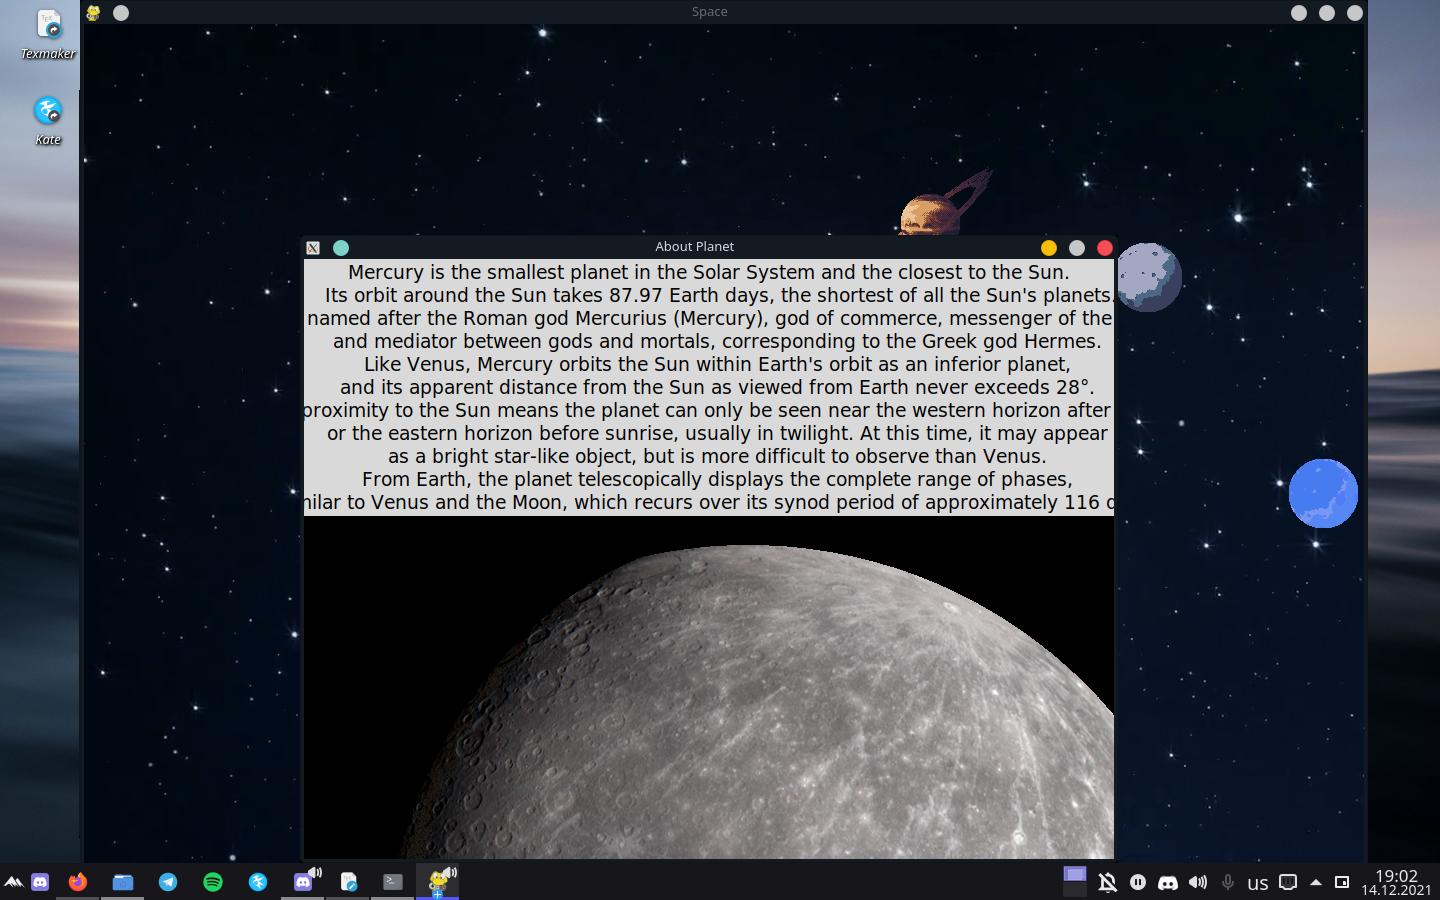
\includegraphics[scale=0.45]{test2} 
\caption{Инф. сообщение}
\end{center}
\end{figure}
\chapter*{Заключение}
\addcontentsline{toc}{section}{Заключение}
В результате данной лабораторной работы был создан программный продукт с красивым пользовательским интерфейсом, который без проблем запускается на операционных системах линейки Linux. 

Программный продукт реализован в среде разработки Pycharm Professional на языке программирования Python3. 

Данное приложение занимает 3.5 мб. Помимо кода программы с ней поставляются изображения для моделирования и словарь с информацией о планетах. 

Результатом работы программы является моделирование солнечной системы с выводом информации о планетах.



\newpage
\addcontentsline{toc}{chapter}{Список использованной литературы}
\printbibliography[title={Список использованной литературы}]

\chapter*{Приложение}
\addcontentsline{toc}{section}{Приложение}
\subsection*{Ссылка на репозиторий}
\texttt{https://github.com/lilbudek/space}
\subsection*{Код программы}
{\scriptsize
\begin{verbatim}
import math
import os
from tkinter import *
from PIL import ImageTk, Image
import pygame
import info

# some constant
WIDTH = 1280
HEIGHT = 960
BLACK = (0, 0, 0)
game_folder = os.path.dirname(__file__)
sprite_folder = os.path.join(game_folder, "resources")


def info_win(number):
    """
    This module is responsible for information about the planets
    """
    tkwin = Tk()
    tkwin.geometry("810x600+300+300")
    tkwin.resizable(False, False)
    tkwin.title("About Planet")
    img = Image.open(os.path.join(sprite_folder, str(number) + "_.jpg"))
    resize_img = img.resize((450, 450))
    small_img = ImageTk.PhotoImage(resize_img)
    picture = Label(image=small_img)
    text = Label(tkwin, text=info.planet_info[number], fg="black", font="none 14 ", anchor=CENTER)
    text.pack()
    picture.pack()
    tkwin.mainloop()


class Planet(pygame.sprite.Sprite):
    """
    Base class of all planets
    args:
        number - planet number
        speed - planet speed
        image - planet image
        rect - the described square
        angle - starting angle of the planet
    """
    def __init__(self, number, velocity, start_pos, a, b):
        """
        planet construction
        """
        pygame.sprite.Sprite.__init__(self)
        self.number = number
        self.speed = velocity
        self.image = pygame.image.load(
            os.path.join(sprite_folder, str(number) + ".png")).convert()
        self.rect = self.image.get_rect()
        self.image.set_colorkey(BLACK)
        self.angle = start_pos
        self.a = a
        self.b = b

    def update(self):
        """
        planet moving
        """
        if self.number == 2:
            self.angle += self.speed
        else:
            self.angle -= self.speed
        if self.angle >= 360:
            self.angle = 0
        self.rect.centerx = self.a * math.cos(self.angle) + WIDTH / 2
        self.rect.centery = self.b * math.sin(self.angle) + HEIGHT / 2


# Create win init application
pygame.init()
screen = pygame.display.set_mode((WIDTH, HEIGHT))
pygame.display.set_caption("Space")

bg = pygame.image.load(os.path.join(sprite_folder, "bg.jpg")).convert()

# hold one cycle time
clock = pygame.time.Clock()

# combine all the pictures into a single group
all_sprites = pygame.sprite.Group()

# make the sun
sun = pygame.image.load(os.path.join(sprite_folder, "0.png")).convert()
sun.set_colorkey(BLACK)
sun_rect = sun.get_rect()
sun_rect.center = (WIDTH / 2, HEIGHT / 2)

planet = [
    Planet(1, 0.00684, 235, 110, 65),
    Planet(2, 0.00348, 346, 150, 95),
    Planet(3, 0.00122, 56, 200, 130),
    Planet(4, 0.00049, 98, 240, 170),
    Planet(5, 0.0000758, 234, 310, 240),
    Planet(6, 0.0000415, 43, 430, 320),
    Planet(7, 0.0000256, 12, 520, 390),
    Planet(8, 0.0000100, 0, 600, 500),
]

# add all generated planet to sprite list
for i in planet:
    all_sprites.add(i)

# Main game cycle
main_loop = True
while main_loop:
    clock.tick(60)   # Fps!!0)1))!0!)))!
    # check all invents
    for event in pygame.event.get():
        # close the window by clicking on the cross
        if event.type == pygame.QUIT:
            main_loop = False
        # open information window when clicked on planet
        if event.type == pygame.MOUSEBUTTONDOWN:
            for obj in planet:
                if obj.rect.collidepoint(pygame.mouse.get_pos()):
                    info_win(obj.number)
    # rendering new frame
    all_sprites.update()
    screen.blit(bg, (0, 0))
    screen.blit(sun, sun_rect)
    all_sprites.draw(screen)
    pygame.display.flip()
pygame.quit()
\end{verbatim}
}

\end{document}

